\chapter{The Menthal Backend (Speed) Architecture}
\label{chap:menthal_backend_architecture}

TODO: introduction

\section{Requirements analysis [SP]}
To determine the Menthal functional and non-functional requirements, first of all we need to formulate its use cases.
Figure~\ref{fig:menthal_use_case_diagram} represents the Use case diagram of Menthal project.
The system consists of two main parts, the client and the server.
This already gives a separation among its users.
On the one side, a user interact with a client application.
Menthal tracks the user behavior and provides a feedback, that is based on the gathered data analysis.
On the other side, system administrators and scientists interact with a server part.
Scientists carry on researches, analysing the obtained information.
A system administrator maintains the system, controls event processing and performes new analysis required by scientists.

\begin{figure}[h]
  \centering
  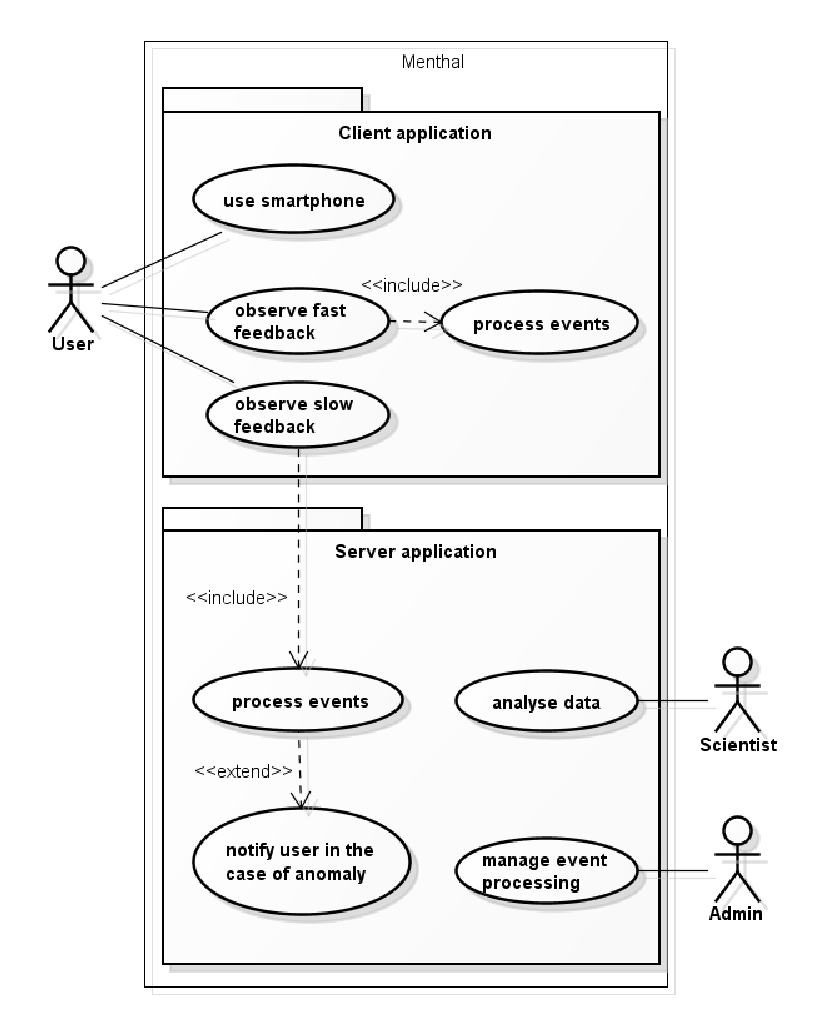
\includegraphics [width=0.9\textwidth]{images/menthal_use_case_diagram}
  \caption{Menthal Use case diagram}
  \label{fig:menthal_use_case_diagram}
\end{figure}


\subsection{Functional requirements}
% to analyze speed layer architecture
The scope of our work is a part of Lambda Architecture named a Speed Layer.
% it consists o three components
% three parts for: receivivg data, ..
It requires to implement three main parts: data receiving part, real-time data processing and the store of the results of computations.
The data receiving part does not need to provide any feedback except the acknoledgement that the data was succeessfully received.
Thus on this end of the system we do not need any special API.
On the contrary, the results of computations can be used further by the other components of the Lambda architecture.
Therefore it can be useful to provide an API that allows to request the necessary information.

% ��������� ����� ��� speed layer, ���� �� ��� ��� ��� ��������?
% or give a big picture (how data goes)


\mnote{Event receiving}
The data receiving part collects the data that arrives from a message queue.
This data consists of various events that represent the actions a user performs on its smartphone. 
The responsibility of the data receiver is to deserialize incoming messages, identify the types of events and let the processing part to handle them.

\mnote{Aggregations}
The processing part of the Speed Layer performs various aggregations on the incoming data.
The distinctive feature of the Speed Layer is that it works only with limited amount of data, processing only the recent events.
Hence it can calculate aggregations and perform analisys in real time.
The created aggregations have different granularities and characterize the different aspects of user-smartphone interaction.

\mnote{Anomaly detection}
As the events are analyzed in real time, it gives an advantage of detecting various anomalies in incoming data.
We should use an appropriate anomaly detection algorithm that can be applied for the given data.
The system should detect the strange behavior in proper time and immediately notify a user if needed.

\mnote{Results storage}
The results of aggregations are stored while the Batch layer of the Lambda architecture performs its calculations.
During this time they should be available for queries.
Our system should provide an API for these purposes.
When the results of aggreagtions are collected from the Speed Layer and merged with the results from the Batch Layer, they can be deleted from a storage.
 
\subsection{Non-functional requirements}
\mnote{Dependency on other components}
The Speed Layer as a part of the Lambda Architecture in particular and the Menthal project in general, needs to be designed taking into account its dependency on other system components
On the one hand, it should follow the principle of modularity, i.e. be self-contained.
Thus, when other parts of the system change, it should not influence the Speed Layer inner structure.
On the other hand, it should be flexible.
In the case of significant changes in the whole system, the adaptation process to the new environment should be fast and easy.

\mnote{Documentation}
All the available features of the Speed Layer should be well documented.
As other parts of the system are maintained by other developers, it is necessary to provide them with the most detailed and relevant description of the system.
It should be easy to obtain necessary information about the system capabilities, where to find the needed functional and how to use it.
Also it is important to provide a convenient mechanism for interpreting the occurring errors. 	    

\mnote{Extensibility}
The system must be easy extendable by additional functionalities.
From the technical side, the Speed Layer consists of a number of cooperating technologies.
These third-party technologies actively develop, the versions of software upgrade.
Therefore our system should allow easy upgrading of its components without a threat of failure.
From the application side, the Menthal project has a great development potential.
New features are constantly added, the functionality is expanded.

\mnote{Security}
Our system needs to meet high security requirement.
Menthal works with user data and stores personal information of real people.
Therefore it is important to protect the stored information from unauthorized access.
The source of information is a smartphone, that transfers collected data to the server.
The data store on the phone and the communication channel should be protected properly.
However, the security problems of these parts of the system are beyond the scope of our work.
We should provide a secure storage system for the results of aggregations, made on the received user data.
Furthermore, only authorized parties can get an access to these results.

\mnote{Performance}
As the Speed Layer should provide the results of data processing in real time, it puts one more requirement on our system.
It should have good performance characteristics.
In our case the costs of processing cores, physical memory and therefore the number of machines needed to perform calculations is less significant than the system performance.
It should work with the fixed and relatively small response time. 

\mnote{Availability and Reliability}
The system must be available and reliable.
The Speed Layer is the only component that has calculated aggregations on the latest data.
Moreover, for anomaly detection purposes it is important not to miss the significant changes in incoming data and react to them in a timely manner.
Therefore, the system should tend to be always available to provide the results of the performed aggregations.
Also it should constantly process the incoming data without failing to avoid the loss of the significant changes that are needed for anomaly detection. 

\mnote{Fault tolerance}
A real-time system should be fault tolerant.
In the case of Speed Layer it is especially relevant, because it consists of many cooperating components.
Even if several nodes in the cluster crash, it should not break the whole system and interrupt the calculation process.
For example, if the server receives the irrelevant event or the message is broken, it should notify about the problem adding an appropriate message into the log file.
However, this incident in no circumstances can be the reason of the whole system crash.
Furthermore, the Speed Layer should have small recovery time in the case of failure. 

\mnote{Efficiency}
We use commodity machines to construct the cluster where the server part of Menthal runs.
Thus it is necessary for our system to be highly efficient.
It should use the given resources in a proper way, allowing other components of the server part run on the same cluster in the full extend.

\mnote{Scalability}
The system load in the Menthal project depends on two main factors.
First, the increasing number of users auguments the load.
This can happen with the growth of popularity of the Menthal application.
Second, the variety of gathered information about user can be extended.
Hence our system should meet the requirement of scalability.
It should be possible to easily add new nodes in the cluster in the case of increasing load.  

\mnote{Codability}
During the development we should take into account the codability of the given system.
The amount of the required man-hours to finish the project is an important indicator of a well thought-out system.
In our case there are several different ways to implement the Speed Layer.
Having the same result, some of them require more effort from a programmer than the others.
It is necessary to choose a right strategy to create a working system.

\mnote{Maintainability}
Our goal is to build a working Speed Layer, however later other people will maintain it and perform the further development.
Thus the maintainability of our system is a significant requirement.
It should be easily configurable.
It need to provide a convenient mechanism to perform the tracking of the running tasks, e.g. using log files.
Finally, our system should have necessary tools for testing its functionality.

These requirements vary in their origins, goals and realisation complexity.
For example, scalability and extensibility are the essential properties of any distributed system.
The real-time processing requires availability, reliability and fault tolerance.
The maintainability and good documentation are easily reachable, they only need a proper approach for software development process.
On the contrary, such requirements as high security and good performance can be hard to implement.
In our work we tried to meet most of these requierements.  

\section{Design of the system [VI]}
Architecture - general schema (picture)
9 pages

\section{Data pipeline (from where to where)}
General schema (picture)
3 pages

kafka + storm + redis

\section{Algorithms}

\section{Mapping to hardware}
how many servers, characteristics, data transferring
1 page

\authorsection{Aspects of implementation}{NO}
programming languages, etc.
